\documentclass{standalone}
\usepackage{tikz}
\usetikzlibrary{patterns, positioning}

\begin{document}
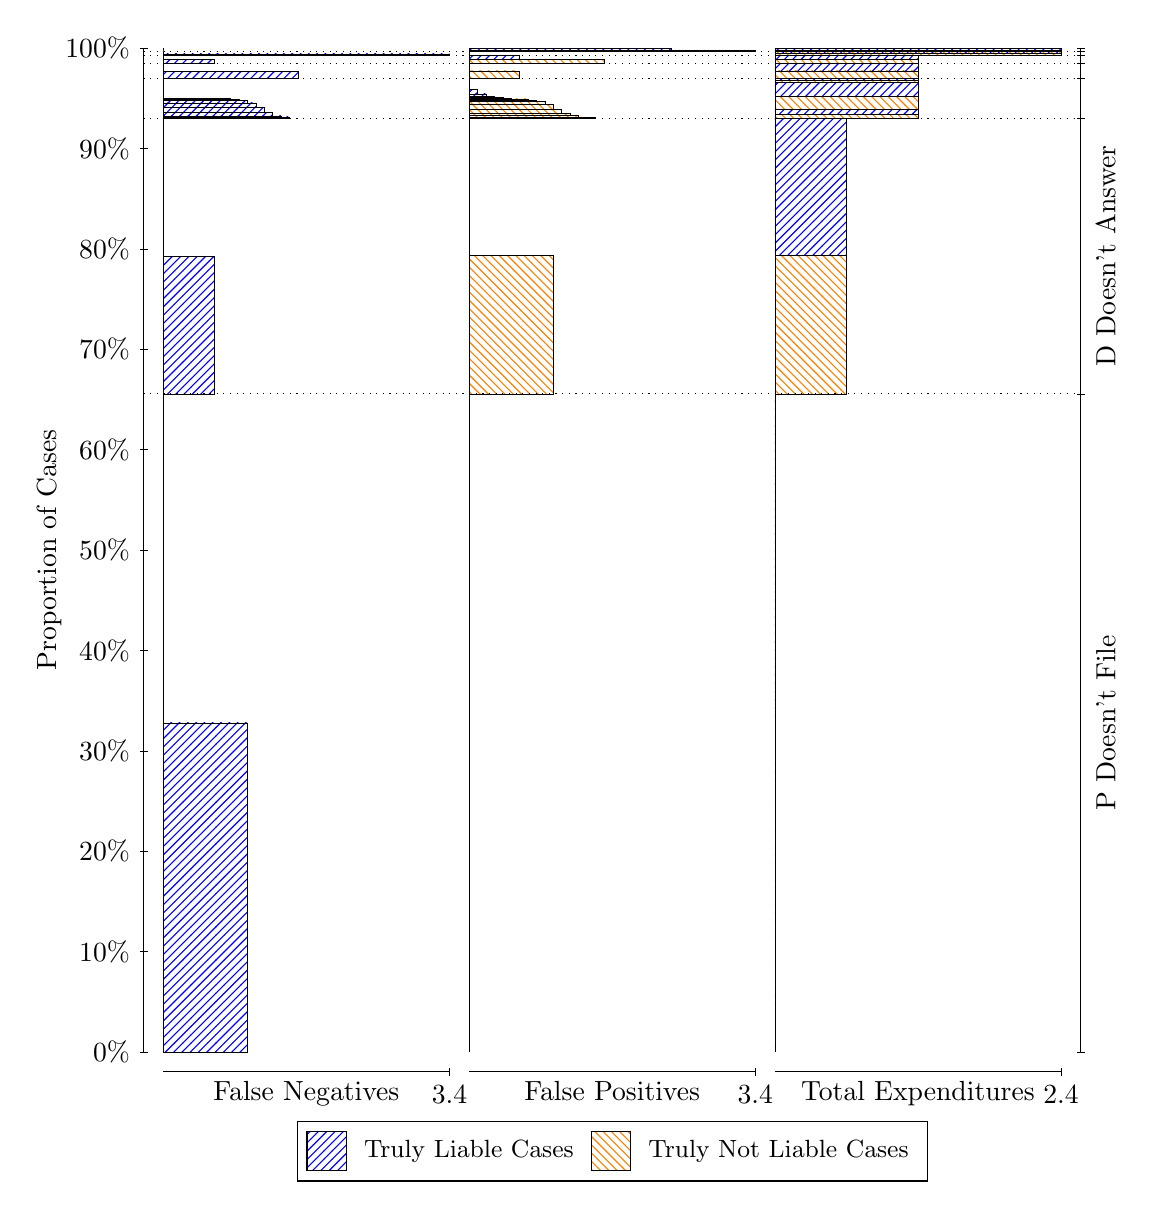
\begin{tikzpicture}
\draw[black, very thin] (1.5,1.75) -- (1.5,14.5);
\node[rotate=90, anchor=center] at (0.3, 8.125) {Proportion of Cases};
\draw[black, very thin] (1.45,1.75) -- (1.55,1.75);
\node[anchor=east] at (1.45, 1.75) {0\%};
\draw[black, very thin] (1.45,3.025) -- (1.55,3.025);
\node[anchor=east] at (1.45, 3.025) {10\%};
\draw[black, very thin] (1.45,4.3) -- (1.55,4.3);
\node[anchor=east] at (1.45, 4.3) {20\%};
\draw[black, very thin] (1.45,5.575) -- (1.55,5.575);
\node[anchor=east] at (1.45, 5.575) {30\%};
\draw[black, very thin] (1.45,6.85) -- (1.55,6.85);
\node[anchor=east] at (1.45, 6.85) {40\%};
\draw[black, very thin] (1.45,8.125) -- (1.55,8.125);
\node[anchor=east] at (1.45, 8.125) {50\%};
\draw[black, very thin] (1.45,9.4) -- (1.55,9.4);
\node[anchor=east] at (1.45, 9.4) {60\%};
\draw[black, very thin] (1.45,10.675) -- (1.55,10.675);
\node[anchor=east] at (1.45, 10.675) {70\%};
\draw[black, very thin] (1.45,11.95) -- (1.55,11.95);
\node[anchor=east] at (1.45, 11.95) {80\%};
\draw[black, very thin] (1.45,13.225) -- (1.55,13.225);
\node[anchor=east] at (1.45, 13.225) {90\%};
\draw[black, very thin] (1.45,14.5) -- (1.55,14.5);
\node[anchor=east] at (1.45, 14.5) {100\%};

\draw[black, very thin] (13.4,1.75) -- (13.4,14.5);
\draw[black, very thin] (13.35,1.75) -- (13.45,1.75);
\node[anchor=west] at (13.35, 1.75) {};
\draw[black, very thin] (13.35,10.107) -- (13.45,10.107);
\node[anchor=west] at (13.35, 10.107) {};
\draw[black, very thin] (13.35,13.609) -- (13.45,13.609);
\node[anchor=west] at (13.35, 13.609) {};
\draw[black, very thin] (13.35,14.111) -- (13.45,14.111);
\node[anchor=west] at (13.35, 14.111) {};
\draw[black, very thin] (13.35,14.306) -- (13.45,14.306);
\node[anchor=west] at (13.35, 14.306) {};
\draw[black, very thin] (13.35,14.409) -- (13.45,14.409);
\node[anchor=west] at (13.35, 14.409) {};
\draw[black, very thin] (13.35,14.455) -- (13.45,14.455);
\node[anchor=west] at (13.35, 14.455) {};
\draw[black, very thin] (13.35,14.5) -- (13.45,14.5);
\node[anchor=west] at (13.35, 14.5) {};

\draw[black, very thin, pattern color=blue, pattern=north east lines] (1.75,1.75) rectangle (2.8186,5.9287);
\draw[black, very thin, pattern color=orange, pattern=north west lines] (1.75,5.9287) rectangle (1.75,10.107);
\draw[black, very thin, pattern color=blue, pattern=north east lines] (1.75,10.107) rectangle (2.3912,11.853);
\draw[black, very thin, pattern color=orange, pattern=north west lines] (1.75,11.853) rectangle (1.75,13.609);
\draw[black, very thin, pattern color=blue, pattern=north east lines] (1.75,13.609) rectangle (3.3529,13.626);
\draw[black, very thin, pattern color=blue, pattern=north east lines] (1.75,13.626) rectangle (3.2461,13.637);
\draw[black, very thin, pattern color=blue, pattern=north east lines] (1.75,13.637) rectangle (3.1392,13.686);
\draw[black, very thin, pattern color=blue, pattern=north east lines] (1.75,13.686) rectangle (3.0324,13.747);
\draw[black, very thin, pattern color=blue, pattern=north east lines] (1.75,13.747) rectangle (2.9255,13.803);
\draw[black, very thin, pattern color=blue, pattern=north east lines] (1.75,13.803) rectangle (2.8186,13.833);
\draw[black, very thin, pattern color=blue, pattern=north east lines] (1.75,13.833) rectangle (2.7118,13.851);
\draw[black, very thin, pattern color=blue, pattern=north east lines] (1.75,13.851) rectangle (2.6049,13.858);
\draw[black, very thin, pattern color=blue, pattern=north east lines] (1.75,13.858) rectangle (2.498,13.865);
\draw[black, very thin, pattern color=orange, pattern=north west lines] (1.75,13.865) rectangle (1.75,14.111);
\draw[black, very thin, pattern color=blue, pattern=north east lines] (1.75,14.111) rectangle (3.4598,14.207);
\draw[black, very thin, pattern color=orange, pattern=north west lines] (1.75,14.207) rectangle (1.75,14.306);
\draw[black, very thin, pattern color=blue, pattern=north east lines] (1.75,14.306) rectangle (2.3912,14.359);
\draw[black, very thin, pattern color=orange, pattern=north west lines] (1.75,14.359) rectangle (1.75,14.409);
\draw[black, very thin, pattern color=blue, pattern=north east lines] (1.75,14.409) rectangle (5.3833,14.425);
\draw[black, very thin, pattern color=orange, pattern=north west lines] (1.75,14.425) rectangle (1.75,14.455);
\draw[black, very thin, pattern color=orange, pattern=north west lines] (1.75,14.455) rectangle (1.75,14.471);
\draw[black, very thin, pattern color=blue, pattern=north east lines] (1.75,14.471) rectangle (1.75,14.5);
\draw[black, very thin, pattern color=orange, pattern=north west lines] (5.6333,1.75) rectangle (5.6333,5.9287);
\draw[black, very thin, pattern color=blue, pattern=north east lines] (5.6333,5.9287) rectangle (5.6333,10.107);
\draw[black, very thin, pattern color=orange, pattern=north west lines] (5.6333,10.107) rectangle (6.702,11.864);
\draw[black, very thin, pattern color=blue, pattern=north east lines] (5.6333,11.864) rectangle (5.6333,13.609);
\draw[black, very thin, pattern color=orange, pattern=north west lines] (5.6333,13.609) rectangle (7.2363,13.616);
\draw[black, very thin, pattern color=orange, pattern=north west lines] (5.6333,13.616) rectangle (7.1294,13.624);
\draw[black, very thin, pattern color=orange, pattern=north west lines] (5.6333,13.624) rectangle (7.0225,13.642);
\draw[black, very thin, pattern color=orange, pattern=north west lines] (5.6333,13.642) rectangle (6.9157,13.672);
\draw[black, very thin, pattern color=orange, pattern=north west lines] (5.6333,13.672) rectangle (6.8088,13.725);
\draw[black, very thin, pattern color=orange, pattern=north west lines] (5.6333,13.725) rectangle (6.702,13.78);
\draw[black, very thin, pattern color=orange, pattern=north west lines] (5.6333,13.78) rectangle (6.5951,13.826);
\draw[black, very thin, pattern color=orange, pattern=north west lines] (5.6333,13.826) rectangle (6.4882,13.836);
\draw[black, very thin, pattern color=orange, pattern=north west lines] (5.6333,13.836) rectangle (6.3814,13.854);
\draw[black, very thin, pattern color=blue, pattern=north east lines] (5.6333,13.854) rectangle (6.1676,13.861);
\draw[black, very thin, pattern color=blue, pattern=north east lines] (5.6333,13.861) rectangle (6.0608,13.869);
\draw[black, very thin, pattern color=blue, pattern=north east lines] (5.6333,13.869) rectangle (5.9539,13.887);
\draw[black, very thin, pattern color=blue, pattern=north east lines] (5.6333,13.887) rectangle (5.8471,13.917);
\draw[black, very thin, pattern color=blue, pattern=north east lines] (5.6333,13.917) rectangle (5.7402,13.973);
\draw[black, very thin, pattern color=blue, pattern=north east lines] (5.6333,13.973) rectangle (5.6333,14.111);
\draw[black, very thin, pattern color=orange, pattern=north west lines] (5.6333,14.111) rectangle (6.2745,14.21);
\draw[black, very thin, pattern color=blue, pattern=north east lines] (5.6333,14.21) rectangle (5.6333,14.306);
\draw[black, very thin, pattern color=orange, pattern=north west lines] (5.6333,14.306) rectangle (7.3431,14.355);
\draw[black, very thin, pattern color=blue, pattern=north east lines] (5.6333,14.355) rectangle (6.2745,14.409);
\draw[black, very thin, pattern color=orange, pattern=north west lines] (5.6333,14.409) rectangle (5.6333,14.438);
\draw[black, very thin, pattern color=blue, pattern=north east lines] (5.6333,14.438) rectangle (5.6333,14.455);
\draw[black, very thin, pattern color=orange, pattern=north west lines] (5.6333,14.455) rectangle (9.2667,14.471);
\draw[black, very thin, pattern color=blue, pattern=north east lines] (5.6333,14.471) rectangle (8.198,14.5);
\draw[black, very thin, pattern color=orange, pattern=north west lines] (9.5167,1.75) rectangle (9.5167,5.9287);
\draw[black, very thin, pattern color=blue, pattern=north east lines] (9.5167,5.9287) rectangle (9.5167,10.107);
\draw[black, very thin, pattern color=orange, pattern=north west lines] (9.5167,10.107) rectangle (10.425,11.864);
\draw[black, very thin, pattern color=blue, pattern=north east lines] (9.5167,11.864) rectangle (10.425,13.609);
\draw[black, very thin, pattern color=orange, pattern=north west lines] (9.5167,13.609) rectangle (11.333,13.662);
\draw[black, very thin, pattern color=blue, pattern=north east lines] (9.5167,13.662) rectangle (11.333,13.718);
\draw[black, very thin, pattern color=orange, pattern=north west lines] (9.5167,13.718) rectangle (11.333,13.885);
\draw[black, very thin, pattern color=blue, pattern=north east lines] (9.5167,13.885) rectangle (11.333,14.059);
\draw[black, very thin, pattern color=orange, pattern=north west lines] (9.5167,14.059) rectangle (11.333,14.085);
\draw[black, very thin, pattern color=blue, pattern=north east lines] (9.5167,14.085) rectangle (11.333,14.111);
\draw[black, very thin, pattern color=orange, pattern=north west lines] (9.5167,14.111) rectangle (11.333,14.21);
\draw[black, very thin, pattern color=blue, pattern=north east lines] (9.5167,14.21) rectangle (11.333,14.306);
\draw[black, very thin, pattern color=orange, pattern=north west lines] (9.5167,14.306) rectangle (11.333,14.355);
\draw[black, very thin, pattern color=blue, pattern=north east lines] (9.5167,14.355) rectangle (11.333,14.409);
\draw[black, very thin, pattern color=orange, pattern=north west lines] (9.5167,14.409) rectangle (13.15,14.438);
\draw[black, very thin, pattern color=blue, pattern=north east lines] (9.5167,14.438) rectangle (13.15,14.455);
\draw[black, very thin, pattern color=orange, pattern=north west lines] (9.5167,14.455) rectangle (13.15,14.471);
\draw[black, very thin, pattern color=blue, pattern=north east lines] (9.5167,14.471) rectangle (13.15,14.5);
\draw[black, dotted] (1.5,10.107) -- (13.4,10.107);
\draw[black, dotted] (1.5,13.609) -- (13.4,13.609);
\draw[black, dotted] (1.5,14.111) -- (13.4,14.111);
\draw[black, dotted] (1.5,14.306) -- (13.4,14.306);
\draw[black, dotted] (1.5,14.409) -- (13.4,14.409);
\draw[black, dotted] (1.5,14.455) -- (13.4,14.455);
\draw[black, very thin] (1.75,1.5) -- (5.3833,1.5);
\node[anchor=north] at (3.5667, 1.5) {False Negatives};
\draw[black, very thin] (5.3833,1.45) -- (5.3833,1.55);
\node[anchor=north] at (5.3833, 1.45) {3.4};

\draw[black, very thin] (5.6333,1.5) -- (9.2667,1.5);
\node[anchor=north] at (7.45, 1.5) {False Positives};
\draw[black, very thin] (9.2667,1.45) -- (9.2667,1.55);
\node[anchor=north] at (9.2667, 1.45) {3.4};

\draw[black, very thin] (9.5167,1.5) -- (13.15,1.5);
\node[anchor=north] at (11.333, 1.5) {Total Expenditures};
\draw[black, very thin] (13.15,1.45) -- (13.15,1.55);
\node[anchor=north] at (13.15, 1.45) {2.4};

\node[black, centered, rotate=90] at (13.72, 5.9287) {P Doesn't File};
\node[black, centered, rotate=90] at (13.72, 11.858) {D Doesn't Answer};






\draw (7.449999999999999,1.5) node[draw=none] (baseCoordinate) {};
\begin{scope}[align=center]
        \matrix[scale=0.5, draw=black, below=0.5cm of baseCoordinate, nodes={draw}, column sep=0.1cm]{
            \node[rectangle, draw, minimum width=0.5cm, minimum height=0.5cm, pattern=north east lines, pattern color=blue] {}; &
            \node[draw=none, font=\small] (B) {Truly Liable Cases}; &
            \node[rectangle, draw, minimum width=0.5cm, minimum height=0.5cm, pattern=north west lines, pattern color=orange] {}; &
            \node[draw=none, font=\small] (B) {Truly Not Liable Cases}; \\
            };
\end{scope}

\end{tikzpicture}
\end{document}